\documentclass[oneside]{article}

% ---------------------------------------------
% Importing packages
% ---------------------------------------------

% Encoding and font
\usepackage[utf8]{inputenc}
\usepackage{tgcursor}
\usepackage{hyperref}

% Different colors
\usepackage{xcolor}
\usepackage{color}
\definecolor{bluepoli}{cmyk}{0.4,0.1,0,0.4}

% Math
\usepackage{amsmath}
\usepackage{amsthm}

% Images
\usepackage{graphicx}
% \graphicspath{ {./Figures/} }

% Margins
\usepackage[a4paper, top=2cm, left=2.5cm, right=2.5cm, bottom=2cm]{geometry}

% Fancy header and footer
\usepackage{fancyhdr}
\pagestyle{fancy}
\fancyhf{}
\rhead{Calcoli di Processo dell'Ingegneria Chimica}
\lhead{Practical Session 5}
\rfoot{Page \thepage}
\lfoot{Academic Year 2024-2025}


\usepackage{amsthm}
\usepackage{tcolorbox}
\tcbuselibrary{most}
\tcolorboxenvironment{proof}{% `proof' from `amsthm'
   blanker,
   breakable,
   left=5mm,
   before skip=10pt,
   after skip=10pt,
   borderline west={1mm}{0pt}{bluepoli}
}

% ---------------------------------------------
% Title
% ---------------------------------------------

\title{Non Linear System of Equations}
\author{Timoteo Dinelli\footnote{timoteo.dinelli@polimi.it}, Marco Mehl\footnote{marco.mehl@polimi.it}}
\date{14\textsuperscript{th} of November 2024}

% ---------------------------------------------
% Begin of the document
% ---------------------------------------------

\begin{document}
\maketitle
% \section{``Boeing 737''}
% Un Boeing 737 tocca la pista d'atterraggio ad una velocità $v = 210 \frac{km}{h}$.
% Vengono subito attivati gli inversori di spinta per deviare i gas di scarico dell'aereo
% nella stessa direzione del moto, ottenendo di conseguenza un'azione frenante. Si chiede
% di calcolare la velocità d'uscita dei gas di scarico (relativa) che permette all'aereo di
% fermarsi in un tempo $t = 15 \: s$.
%
% \subsection*{Dati:}
% \begin{itemize}
%    \item massa iniziale BOEING = 35000 $kg$
%    \item f = 0.97
%    \item Sezione d'uscita gas di scarico = 0.085 $m^{2}$
%    \item Area frontale investita dall'aria = 25 $m^{2}$
% \end{itemize}
%
% \subsection*{Soluzione:}
% \begin{align}
%    \frac{d(mv)}{dt} &= -2\dot{m}_{out} v_{out} - \frac{1}{2} f \rho v^{2} A \\
%    m\frac{dv}{dt} &= -2\dot{m}_{out} (v_{out} - v) - \frac{1}{2} f \rho v^{2} A \\
%    m\frac{dv}{dt} &= -2 \dot{m}_{out} v_{r} - \frac{1}{2} f \rho v^{2} A \\
%    m(t) &= m_{0} - 2\dot{m} t \\
%    (m_{0} - 2\dot{m}_{out} t )\frac{dv}{dt} &= -2\dot{m}_{out} v_{r} - \frac{1}{2} f \rho
%    v^{2} A
% \end{align}
% \begin{align}
%    \int_{v_{0}}^{0}\frac{dv}{2\dot{m}_{out} v_{r} + \frac{1}{2} f v^{2} A} &=-
%    \int_{0}^{t} \frac{dt}{m_{0} - 2\dot{m}_{out} t} \\
%    \dot{m}_{out} &= \rho S v_{r} \\
%    \int_{v_{0}}^{0}\frac{dv}{2 S v_{r}^{2} + \frac{1}{2} f v^{2} A} &=-\rho \int_{0}^{t}
%    \frac{dt}{m_{0} - 2\rho S v_{r} t}
% \end{align}
% \begin{equation*}
%    \alpha = 2 S v_{r}^{2}, \quad \beta = \frac{1}{2} f A, \quad \gamma = m_{0}, \quad
%    \delta = 2 \rho S v_{r}.
% \end{equation*}
%
% \begin{align}
%    \int_{v_{0}}^{0} \frac{dv}{\alpha + \beta v^{2}} &= -\rho \int_{0}^{t}
%    \frac{dt}{\gamma - \delta t} \\
%    \int \frac{1}{\alpha + \beta x^{2}} dx &=
%    \frac{atan\left(\sqrt{x\frac{\beta}{\alpha}}\right)}{\sqrt{\alpha \beta}} + c \\
%    \int \frac{1}{\gamma - \delta x} dx &= -\frac{log\left(\gamma - \delta
%    x\right)}{\delta} + c
% \end{align}
% \begin{equation}
%    \label{eq:final}
%    \frac{1}{\sqrt{\alpha\beta}} atan\left( v_{0} \sqrt{\frac{\beta}{\alpha}}\right) +
%    \frac{\rho}{\delta}ln\left(1-\frac{\delta}{\gamma}t\right) = 0
% \end{equation}
%
% Rearrange equation number \ref{eq:final} as to be $\delta = ...$, after some simple steps
% we obtain:
%
% \begin{equation}
%    \delta = \frac{\gamma}{t}\left(1-exp\left(-\frac{\delta}{\rho \sqrt{\alpha \beta}}
%    atan\left(v_{0}\sqrt{\frac{\beta}{\alpha}}\right)\right)\right)
% \end{equation}
% \begin{equation*}
%    \delta = 2 \rho S v
% \end{equation*}
% \begin{equation}
%    v = \frac{\gamma}{2 \rho S t}\left(1-exp\left(-\frac{\delta}{\rho \sqrt{\alpha \beta}}
%       atan\left(v_{0}\sqrt{\frac{\beta}{\alpha}}\right)\right)\right)
% \end{equation}

\section{``Bacini comunicanti con perdite di carico''}
\begin{figure}[htp]
   \centering
   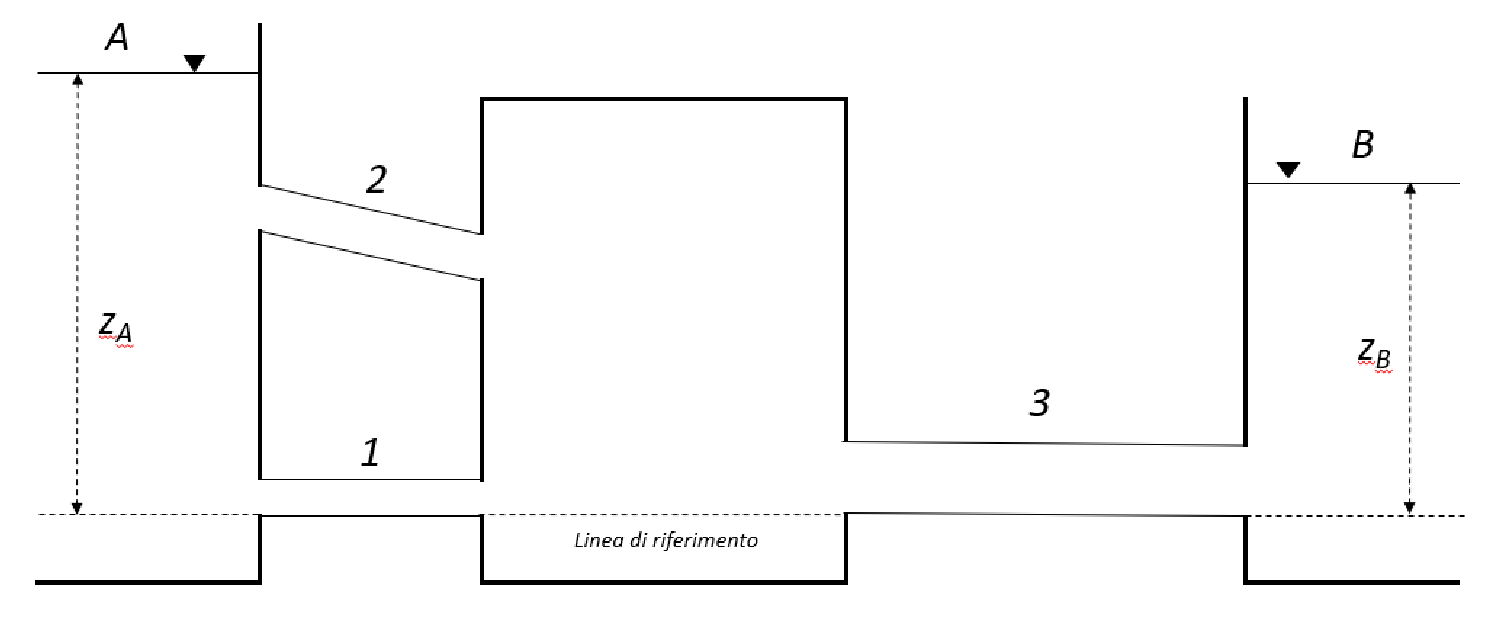
\includegraphics[width=.8\textwidth]{Tanks.png}
   \caption{Schematizzazione del sistema di collegamento di due serbatoi.}
   \label{fig:fig1}
\end{figure}

Due bacini d’acqua (\textbf{A} e \textbf{B}) sono collegati fra loro con il sistema di
tubazioni rappresentato in figura \ref{fig:fig1}. Dal bacino \textbf{A} partono due
tubazioni (\textit{1} e \textit{2}) di lunghezza e diametro diversi, che si congiungono
in un barilotto dal quale un' unica tubazione (\textit{3}) convoglia l’acqua verso il
bacino \textbf{B}. Le tubazioni \textit{1} e \textit{2} possono essere utilizzate in
alternativa, chiudendone una delle due, o assieme quando entrambe sono aperte. Sulla base
dei dati forniti, si chiede di calcolare la portata quando sono aperti i tubi \textit{1}
e \textit{3}.

\noindent \textbf{Dati}:
\begin{itemize}
   \item $\frac{\epsilon_{1}}{D_1} = \frac{\epsilon_{2}}{D_2} = \frac{\epsilon_{3}}{D_3}
      = 0.001$.
   \item $D_1 = 0.3 \: m$, $L_1 = 300 \: m$.
   \item $D_2 = 0.2 \: m$, $L_2 = 346.4 \: m$.
   \item $D_3 = 0.4 \: m$, $L_3 = 900 \: m$.
   \item $\rho_{H_{2}O} = 1000 \: \frac{kg}{m^3}$.
   \item $\mu_{H_{2}O} = 1.141 \times 10^{-3} \: Pa \: s$.
   \item $z_A = 80 \: m$.
   \item $z_B = 30 \: m$.
   \item Formula di Colebrook-White: $\frac{1}{\sqrt{f}} = -4
      log\left(\frac{\epsilon}{3.7 \: D} + \frac{1.255}{Re \sqrt{f}}\right)$
\end{itemize}

\section*{Soluzione}
A causa delle perdite di carico nelle tubazioni, il trinomio di Bernoulli non si mantiene costante tra i due bacini.
Il bilancio dell’energia meccanica tra i peli liberi dei due bacini risulta:

\begin{align}
   z_A &= z_B + \Delta H_1 + \Delta H_3 \\
   \Delta H_1 &= 4 \frac{L_1}{D_1} f_1 \frac{v_{1}^{2}}{2g} \\
   \Delta H_3 &= 4 \frac{L_3}{D_3} f_3 \frac{v_{3}^{3}}{3g}
\end{align}

Uguagliando le portate nei tubi 1 e 3 si ha:

\begin{equation}
   v_3 = v_1 \left(\frac{D_1}{D_3}\right)^2
\end{equation}

che permette di scrivere il bilancio dell’energia meccanica in funzione della sola
incognita $v_1$:

\begin{equation}\label{eq:final}
   z_A - z_B = \frac{v_{1}^{2}}{2g}\left(4 \frac{L_1}{D_1} f_1 + 4
   \frac{L_3}{D_3}\left(\frac{D_1}{D_3}\right)^4 f_3 \right)
\end{equation}

Si noti tuttavia che l'equazione \ref{eq:final} risulta effetivamente un' unica equazione
funzione dell'incognita $v_1$ tuttavia $f_1$ e $f_3$ dipendono implicitamente da $v_1$
pertanto risulta necessario risolvere (numericamente) il seguente sistema di equazioni
nelle tre incognite $Q = \frac{v_{1, 3}}{\frac{\pi D_{1,3}^2}{4}}$, $f_1$, $f_3$:

\begin{equation}
   \begin{cases}
      z_A - \left(z_B  + \Delta H_1 + \Delta H_3 \right) &= 0 \\
      \frac{1}{\sqrt{f_1}} - \left(-4 log\left(\frac{\epsilon}{3.7 \: D} + \frac{1.255}{Re
      \sqrt{f_1}}\right)\right) &= 0 \\
      \frac{1}{\sqrt{f_3}} - \left(-4 log\left(\frac{\epsilon}{3.7 \: D} + \frac{1.255}{Re
      \sqrt{f_3}}\right)\right) &= 0 \\
   \end{cases}
\end{equation}
\end{document}
